\batchmode


\documentclass{jarticle}
\RequirePackage{ifthen}


\usepackage{makeidx,mytabbing,fancyheadings,amsmath}
\usepackage[dvipdfmx]{graphicx}
\usepackage[dvipdfmx,bookmarks=true,bookmarksnumbered=true,bookmarkstype=toc]{hyperref}
\ifnum 42146=\euc"A4A2 \AtBeginDvi{\special{pdf:tounicode EUC-UCS2}}\else
\AtBeginDvi{\special{pdf:tounicode 90ms-RKSJ-UCS2}}\fi

%
\providecommand{\eusversion}{9.22} 


\flushbottom
\makeindex
\pagestyle{myheadings}
\oddsidemargin=0cm
\evensidemargin=0cm


\textwidth=16.5cm
\textheight=24.6cm
\topmargin=-0.8cm
\oddsidemargin= 0.5cm
\evensidemargin=0.5cm


\parindent=10pt
\parskip=1mm


\setcounter{totalnumber}{3}
%
\renewcommand{\topfraction}{0.99}       % 85% of a page (from page
                                        %
\renewcommand{\bottomfraction}{0.99}    % 85% of a page (from page
                                        %
\renewcommand{\textfraction}{0.0}      % text shoud occupy 15% or
                                        



\usepackage[dvips]{color}


\pagecolor[rgb]{1,1,1}

\usepackage[]{inputenc}



\makeatletter

\makeatletter
\count@=\the\catcode`\_ \catcode`\_=8 
\newenvironment{tex2html_wrap}{}{}%
\catcode`\<=12\catcode`\_=\count@
\newcommand{\providedcommand}[1]{\expandafter\providecommand\csname #1\endcsname}%
\newcommand{\renewedcommand}[1]{\expandafter\providecommand\csname #1\endcsname{}%
  \expandafter\renewcommand\csname #1\endcsname}%
\newcommand{\newedenvironment}[1]{\newenvironment{#1}{}{}\renewenvironment{#1}}%
\let\newedcommand\renewedcommand
\let\renewedenvironment\newedenvironment
\makeatother
\let\mathon=$
\let\mathoff=$
\ifx\AtBeginDocument\undefined \newcommand{\AtBeginDocument}[1]{}\fi
\newbox\sizebox
\setlength{\hoffset}{0pt}\setlength{\voffset}{0pt}
\addtolength{\textheight}{\footskip}\setlength{\footskip}{0pt}
\addtolength{\textheight}{\topmargin}\setlength{\topmargin}{0pt}
\addtolength{\textheight}{\headheight}\setlength{\headheight}{0pt}
\addtolength{\textheight}{\headsep}\setlength{\headsep}{0pt}
\setlength{\textwidth}{349pt}
\newwrite\lthtmlwrite
\makeatletter
\let\realnormalsize=\normalsize
\global\topskip=2sp
\def\preveqno{}\let\real@float=\@float \let\realend@float=\end@float
\def\@float{\let\@savefreelist\@freelist\real@float}
\def\liih@math{\ifmmode$\else\bad@math\fi}
\def\end@float{\realend@float\global\let\@freelist\@savefreelist}
\let\real@dbflt=\@dbflt \let\end@dblfloat=\end@float
\let\@largefloatcheck=\relax
\let\if@boxedmulticols=\iftrue
\def\@dbflt{\let\@savefreelist\@freelist\real@dbflt}
\def\adjustnormalsize{\def\normalsize{\mathsurround=0pt \realnormalsize
 \parindent=0pt\abovedisplayskip=0pt\belowdisplayskip=0pt}%
 \def\phantompar{\csname par\endcsname}\normalsize}%
\def\lthtmltypeout#1{{\let\protect\string \immediate\write\lthtmlwrite{#1}}}%
\newcommand\lthtmlhboxmathA{\adjustnormalsize\setbox\sizebox=\hbox\bgroup\kern.05em }%
\newcommand\lthtmlhboxmathB{\adjustnormalsize\setbox\sizebox=\hbox to\hsize\bgroup\hfill }%
\newcommand\lthtmlvboxmathA{\adjustnormalsize\setbox\sizebox=\vbox\bgroup %
 \let\ifinner=\iffalse \let\)\liih@math }%
\newcommand\lthtmlboxmathZ{\@next\next\@currlist{}{\def\next{\voidb@x}}%
 \expandafter\box\next\egroup}%
\newcommand\lthtmlmathtype[1]{\gdef\lthtmlmathenv{#1}}%
\newcommand\lthtmllogmath{\dimen0\ht\sizebox \advance\dimen0\dp\sizebox
  \ifdim\dimen0>.95\vsize
   \lthtmltypeout{%
*** image for \lthtmlmathenv\space is too tall at \the\dimen0, reducing to .95 vsize ***}%
   \ht\sizebox.95\vsize \dp\sizebox\z@ \fi
  \lthtmltypeout{l2hSize %
:\lthtmlmathenv:\the\ht\sizebox::\the\dp\sizebox::\the\wd\sizebox.\preveqno}}%
\newcommand\lthtmlfigureA[1]{\let\@savefreelist\@freelist
       \lthtmlmathtype{#1}\lthtmlvboxmathA}%
\newcommand\lthtmlpictureA{\bgroup\catcode`\_=8 \lthtmlpictureB}%
\newcommand\lthtmlpictureB[1]{\lthtmlmathtype{#1}\egroup
       \let\@savefreelist\@freelist \lthtmlhboxmathB}%
\newcommand\lthtmlpictureZ[1]{\hfill\lthtmlfigureZ}%
\newcommand\lthtmlfigureZ{\lthtmlboxmathZ\lthtmllogmath\copy\sizebox
       \global\let\@freelist\@savefreelist}%
\newcommand\lthtmldisplayA{\bgroup\catcode`\_=8 \lthtmldisplayAi}%
\newcommand\lthtmldisplayAi[1]{\lthtmlmathtype{#1}\egroup\lthtmlvboxmathA}%
\newcommand\lthtmldisplayB[1]{\edef\preveqno{(\theequation)}%
  \lthtmldisplayA{#1}\let\@eqnnum\relax}%
\newcommand\lthtmldisplayZ{\lthtmlboxmathZ\lthtmllogmath\lthtmlsetmath}%
\newcommand\lthtmlinlinemathA{\bgroup\catcode`\_=8 \lthtmlinlinemathB}
\newcommand\lthtmlinlinemathB[1]{\lthtmlmathtype{#1}\egroup\lthtmlhboxmathA
  \vrule height1.5ex width0pt }%
\newcommand\lthtmlinlineA{\bgroup\catcode`\_=8 \lthtmlinlineB}%
\newcommand\lthtmlinlineB[1]{\lthtmlmathtype{#1}\egroup\lthtmlhboxmathA}%
\newcommand\lthtmlinlineZ{\egroup\expandafter\ifdim\dp\sizebox>0pt %
  \expandafter\centerinlinemath\fi\lthtmllogmath\lthtmlsetinline}
\newcommand\lthtmlinlinemathZ{\egroup\expandafter\ifdim\dp\sizebox>0pt %
  \expandafter\centerinlinemath\fi\lthtmllogmath\lthtmlsetmath}
\newcommand\lthtmlindisplaymathZ{\egroup %
  \centerinlinemath\lthtmllogmath\lthtmlsetmath}
\def\lthtmlsetinline{\hbox{\vrule width.1em \vtop{\vbox{%
  \kern.1em\copy\sizebox}\ifdim\dp\sizebox>0pt\kern.1em\else\kern.3pt\fi
  \ifdim\hsize>\wd\sizebox \hrule depth1pt\fi}}}
\def\lthtmlsetmath{\hbox{\vrule width.1em\kern-.05em\vtop{\vbox{%
  \kern.1em\kern0.8 pt\hbox{\hglue.17em\copy\sizebox\hglue0.8 pt}}\kern.3pt%
  \ifdim\dp\sizebox>0pt\kern.1em\fi \kern0.8 pt%
  \ifdim\hsize>\wd\sizebox \hrule depth1pt\fi}}}
\def\centerinlinemath{%
  \dimen1=\ifdim\ht\sizebox<\dp\sizebox \dp\sizebox\else\ht\sizebox\fi
  \advance\dimen1by.5pt \vrule width0pt height\dimen1 depth\dimen1 
 \dp\sizebox=\dimen1\ht\sizebox=\dimen1\relax}

\def\lthtmlcheckvsize{\ifdim\ht\sizebox<\vsize 
  \ifdim\wd\sizebox<\hsize\expandafter\hfill\fi \expandafter\vfill
  \else\expandafter\vss\fi}%
\providecommand{\selectlanguage}[1]{}%
\makeatletter \tracingstats = 1 
\providecommand{\Eta}{\textrm{H}}
\providecommand{\Epsilon}{\textrm{E}}
\providecommand{\Zeta}{\textrm{Z}}
\providecommand{\Beta}{\textrm{B}}
\providecommand{\Nu}{\textrm{N}}
\providecommand{\omicron}{\textrm{o}}
\providecommand{\Tau}{\textrm{T}}
\providecommand{\Omicron}{\textrm{O}}
\providecommand{\Rho}{\textrm{R}}
\providecommand{\Iota}{\textrm{J}}
\providecommand{\Chi}{\textrm{X}}
\providecommand{\Mu}{\textrm{M}}
\providecommand{\Alpha}{\textrm{A}}
\providecommand{\Kappa}{\textrm{K}}


\begin{document}
\pagestyle{empty}\thispagestyle{empty}\lthtmltypeout{}%
\lthtmltypeout{latex2htmlLength hsize=\the\hsize}\lthtmltypeout{}%
\lthtmltypeout{latex2htmlLength vsize=\the\vsize}\lthtmltypeout{}%
\lthtmltypeout{latex2htmlLength hoffset=\the\hoffset}\lthtmltypeout{}%
\lthtmltypeout{latex2htmlLength voffset=\the\voffset}\lthtmltypeout{}%
\lthtmltypeout{latex2htmlLength topmargin=\the\topmargin}\lthtmltypeout{}%
\lthtmltypeout{latex2htmlLength topskip=\the\topskip}\lthtmltypeout{}%
\lthtmltypeout{latex2htmlLength headheight=\the\headheight}\lthtmltypeout{}%
\lthtmltypeout{latex2htmlLength headsep=\the\headsep}\lthtmltypeout{}%
\lthtmltypeout{latex2htmlLength parskip=\the\parskip}\lthtmltypeout{}%
\lthtmltypeout{latex2htmlLength oddsidemargin=\the\oddsidemargin}\lthtmltypeout{}%
\makeatletter
\if@twoside\lthtmltypeout{latex2htmlLength evensidemargin=\the\evensidemargin}%
\else\lthtmltypeout{latex2htmlLength evensidemargin=\the\oddsidemargin}\fi%
\lthtmltypeout{}%
\makeatother
\setcounter{page}{1}
\onecolumn

% !!! IMAGES START HERE !!!

\setcounter{totalnumber}{3}

%
\providecommand{\ptext}[1]{\tt \begin{quote} \begin{tabbing} #1 \end{tabbing} \end{quote} \rm}%


%
\providecommand{\desclist}[1]{
\begin{list}{ }{\setlength{\rightmargin}{0mm}\topsep=0mm\partopsep=0mm}
\item #1
\end{list}
\vspace{3mm}}%


%
\providecommand{\functiondescription}[4]{

{\bf #1} \em #2 \rm \hfill [#3] 

\begin{list}{ }{\setlength{\rightmargin}{0mm}\topsep=0mm\partopsep=0mm}
\item \hspace{0mm}#4
\end{list}
\vspace{3mm}
}%


%
\providecommand{\bfx}[1]{{\bf #1}}%


%
\providecommand{\emx}[1]{{\em #1}}%


%
\providecommand{\longdescription}[3]{

\begin{tabbing}
{\bf #1} 
\it #2
\rm
\end{tabbing}

\begin{list}{ }{\setlength{\rightmargin}{0mm}\topsep=0mm\partopsep=0mm}
\item #3
\end{list}
\vspace{3mm}
}%


%
\providecommand{\funcdesc}[3]{

{\bf #1} \em #2 \rm \hfill [関数] 

\begin{list}{ }{\setlength{\rightmargin}{0mm}\topsep=0mm\partopsep=0mm}
\item \hspace{0mm}#3
\end{list}
\vspace{3mm}
}%


%
\providecommand{\macrodesc}[3]{

{\bf #1} \em #2 \rm \hfill [マクロ] 

\begin{list}{ }{\setlength{\rightmargin}{0mm}\topsep=0mm\partopsep=0mm}
\item \hspace{0mm}#3
\end{list}
\vspace{3mm}
}%


%
\providecommand{\specialdesc}[3]{

{\bf #1} \em #2 \rm \hfill [特殊] 

\begin{list}{ }{\setlength{\rightmargin}{0mm}\topsep=0mm\partopsep=0mm}
\item \hspace{0mm}#3
\end{list}
\vspace{3mm}
}%


%
\providecommand{\methoddesc}[3]{

{\bf #1} \em #2 \rm \hfill [メソッド] 

\begin{list}{ }{\setlength{\rightmargin}{0mm}\topsep=0mm\partopsep=0mm}
\item \hspace{0mm}#3
\end{list}
\vspace{3mm}
}%


%
\providecommand{\vardesc}[2]{

{\bf #1} \em  \rm \hfill [変数] 

\begin{list}{ }{\setlength{\rightmargin}{0mm}\topsep=0mm\partopsep=0mm}
\item \hspace{0mm}#2
\end{list}
\vspace{3mm}
}%


%
\providecommand{\fundesc}[2]{

{\bf #1} \em #2 \rm \hfill [関数] 

\begin{list}{ }{\setlength{\rightmargin}{0mm}\topsep=0mm\partopsep=0mm}
\item \hspace{0mm}\hspace{0mm}
\end{list}
\vspace{3mm}
}%


%
\providecommand{\macdesc}[2]{

{\bf #1} \em #2 \rm \hfill [マクロ] 

\begin{list}{ }{\setlength{\rightmargin}{0mm}\topsep=0mm\partopsep=0mm}
\item \hspace{0mm}\hspace{0mm}
\end{list}
\vspace{3mm}
}%


%
\providecommand{\spedesc}[2]{

{\bf #1} \em #2 \rm \hfill [特殊] 

\begin{list}{ }{\setlength{\rightmargin}{0mm}\topsep=0mm\partopsep=0mm}
\item \hspace{0mm}\hspace{0mm}
\end{list}
\vspace{3mm}
}%


%
\providecommand{\metdesc}[2]{

{\bf #1} \em #2 \rm \hfill [メソッド] 

\begin{list}{ }{\setlength{\rightmargin}{0mm}\topsep=0mm\partopsep=0mm}
\item \hspace{0mm}\hspace{0mm}
\end{list}
\vspace{3mm}
}%


%
\providecommand{\constdesc}[2]{

{\bf #1} \em  \rm \hfill [定数] 

\begin{list}{ }{\setlength{\rightmargin}{0mm}\topsep=0mm\partopsep=0mm}
\item \hspace{0mm}#2
\end{list}
\vspace{3mm}
}%


%
\providecommand{\classdesc}[4]{	%class, super slots description
\vspace{2mm} 

{\Large {\bf #1 }} \hfill [クラス]  %super
\begin{tabbing}
\hspace{30mm} :super \hspace{5mm} \= {\bf #2} \\
\hspace{30mm} :slots \> #3 
\end{tabbing}
\vspace{4mm}

\begin{list}{ }{\setlength{\rightmargin}{0mm}\topsep=0mm\partopsep=0mm}
\item #4
\end{list}
\vspace{3mm}}%



\newedenvironment{refdesc}{
 \vspace{5mm} \parindent=0mm \topsep=0mm \parskip=0mm \leftmargin=10mm}{
             \parindent=10mm \topsep=3mm \parskip=1mm \leftmargin=0mm }%

\stepcounter{part}
\stepcounter{section}
\stepcounter{subsection}
\stepcounter{subsection}
\stepcounter{subsection}
\setcounter{enumi}{3}
\stepcounter{subsection}
\stepcounter{subsection}
\stepcounter{subsection}
\stepcounter{subsection}
{\newpage\clearpage
\lthtmlpictureA{tex2html_wrap56602}%
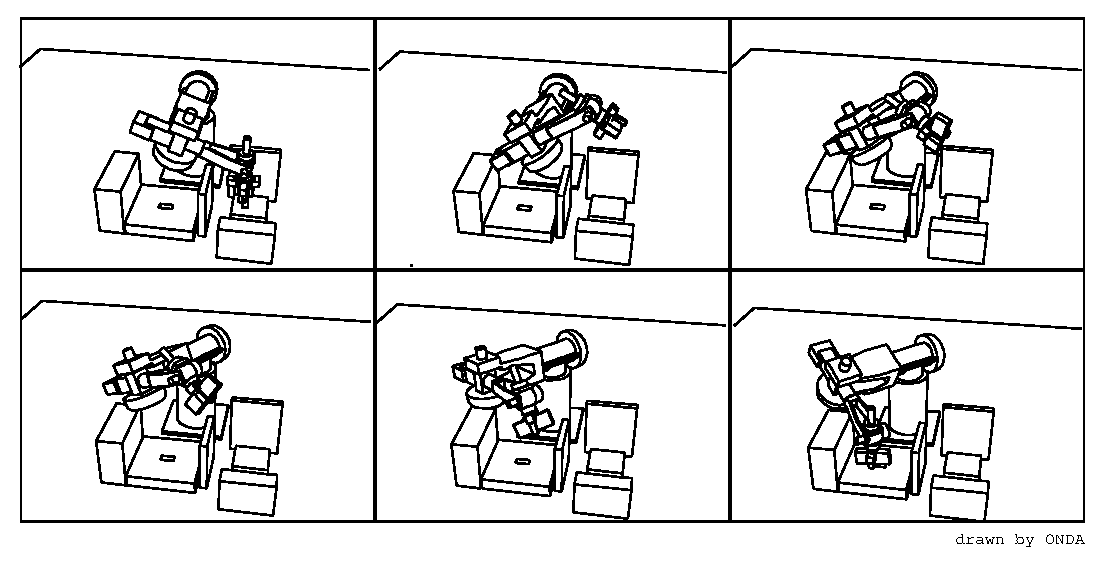
\includegraphics[width=150mm]{fig/eta3colavo.ps}%
\lthtmlpictureZ
\lthtmlcheckvsize\clearpage}

\stepcounter{section}
{\newpage\clearpage
\lthtmlpictureA{tex2html_wrap56604}%
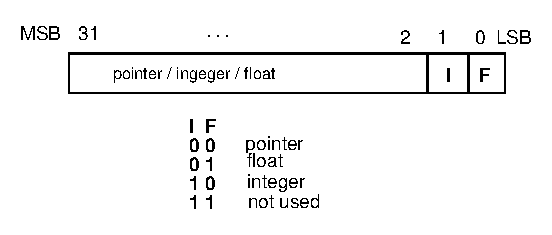
\includegraphics{fig/pointer.ps}%
\lthtmlpictureZ
\lthtmlcheckvsize\clearpage}

\stepcounter{subsection}
\stepcounter{subsection}
{\newpage\clearpage
\lthtmlpictureA{tex2html_wrap56614}%
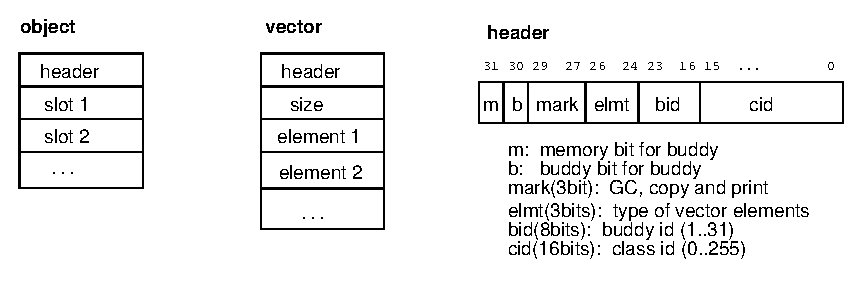
\includegraphics{fig/object.ps}%
\lthtmlpictureZ
\lthtmlcheckvsize\clearpage}

\stepcounter{subsection}
{\newpage\clearpage
\lthtmlfigureA{figure753}%
\begin{figure}\small
\begin{verbatim}

object
     cons
          queue
     propertied-object
          symbol   -----  foreign-pod
          package
          stream
               file-stream
               broadcast-stream
          io-stream ---- socket-stream
          metaclass
               vectorclass
                    cstructclass
          read-table
          array
          thread
          barrier-synch
          synch-memory-port
          coordinates
               cascaded-coords
                    body
                    sphere
                    viewing
                         projection
                              viewing2d
                              parallel-viewing
                              perspective-viewing
                    coordinates-axes
               viewport
          line --- edge --- winged-edge
          plane
               polygon
                    face
                    hole
               semi-space
          viewer
          viewsurface  ----- tektro-viewsurface
     compiled-code
          foreign-code
          closure
          load-module
     label-reference
     vector
          float-vector
          integer-vector
          string
               socket-address
               cstruct
          bit-vector
          foreign-string
     socket-port
     pathname
     hash-table
     surrounding-box
     stereo-viewing\end{verbatim}

\normalsize

\end{figure}%
\lthtmlfigureZ
\lthtmlcheckvsize\clearpage}

\stepcounter{subsection}
\stepcounter{section}
\stepcounter{subsection}
\stepcounter{subsection}
\stepcounter{subsection}
\stepcounter{subsection}
\stepcounter{subsection}
\stepcounter{subsection}
\stepcounter{section}
\stepcounter{subsection}
\stepcounter{subsection}
\stepcounter{subsection}
\stepcounter{subsection}
\stepcounter{subsection}
\stepcounter{subsection}
\stepcounter{section}
\stepcounter{subsection}
\stepcounter{subsection}
\stepcounter{subsection}
\stepcounter{subsection}
\stepcounter{section}
\stepcounter{subsection}
\stepcounter{subsection}
\stepcounter{subsection}
\stepcounter{subsection}
\stepcounter{subsection}
\stepcounter{section}
\stepcounter{subsection}
\stepcounter{subsection}
\stepcounter{section}
\stepcounter{subsection}
\stepcounter{subsection}
\stepcounter{subsection}
\stepcounter{subsection}
\stepcounter{subsubsection}
\stepcounter{subsection}
\stepcounter{subsection}
\stepcounter{subsection}
\stepcounter{section}
\stepcounter{subsection}
\stepcounter{subsection}
\stepcounter{subsection}
\stepcounter{subsection}
\stepcounter{subsubsection}
\stepcounter{subsubsection}
\stepcounter{subsubsection}
\stepcounter{subsection}
\stepcounter{subsection}
\stepcounter{subsection}
\stepcounter{section}
\stepcounter{subsection}
\stepcounter{subsection}
\stepcounter{subsection}
\stepcounter{subsection}
\stepcounter{subsection}
\stepcounter{subsection}
\stepcounter{subsection}
\stepcounter{subsection}
\stepcounter{subsection}
\stepcounter{part}
\stepcounter{section}
\stepcounter{subsection}
\stepcounter{subsection}
\stepcounter{subsubsection}
\stepcounter{subsubsection}
\stepcounter{subsubsection}
\stepcounter{subsubsection}
\stepcounter{subsubsection}
\stepcounter{subsubsection}
\stepcounter{subsubsection}
\stepcounter{subsubsection}
\stepcounter{subsection}
\stepcounter{subsection}
\stepcounter{subsection}
\stepcounter{subsection}
\stepcounter{subsubsection}
\stepcounter{subsubsection}


\setlength{\itemsep}{0cm}%

\setlength{\itemsep}{0cm}
\stepcounter{section}
\stepcounter{subsection}
\stepcounter{subsubsection}
\stepcounter{subsubsection}
{\newpage\clearpage
\lthtmlpictureA{tex2html_wrap57675}%
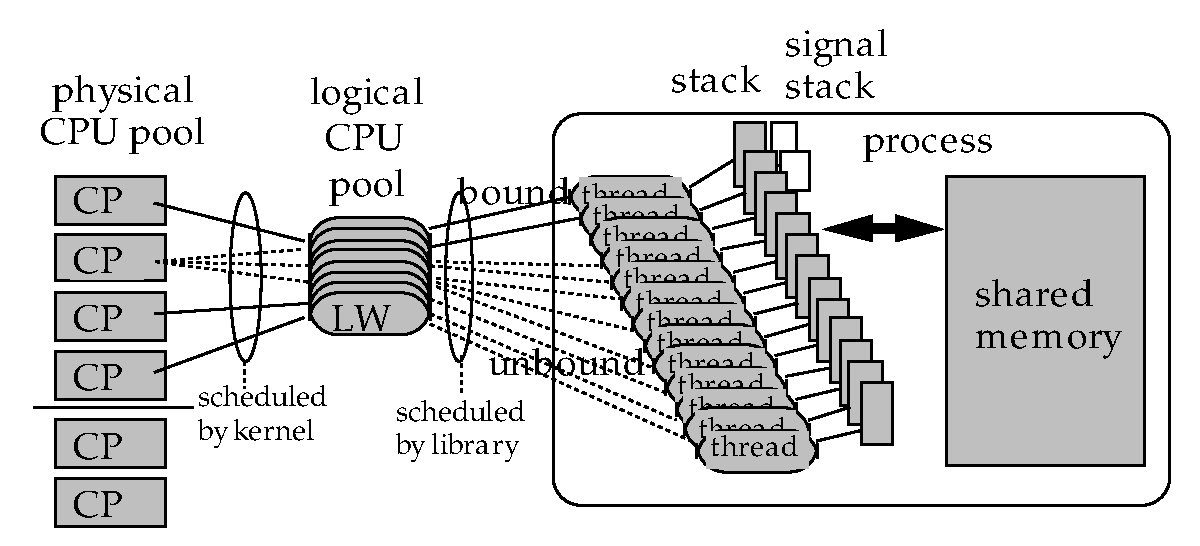
\includegraphics[width=130mm]{fig/threadfig.ps}%
\lthtmlpictureZ
\lthtmlcheckvsize\clearpage}

\stepcounter{subsubsection}
{\newpage\clearpage
\lthtmlpictureA{tex2html_wrap57680}%
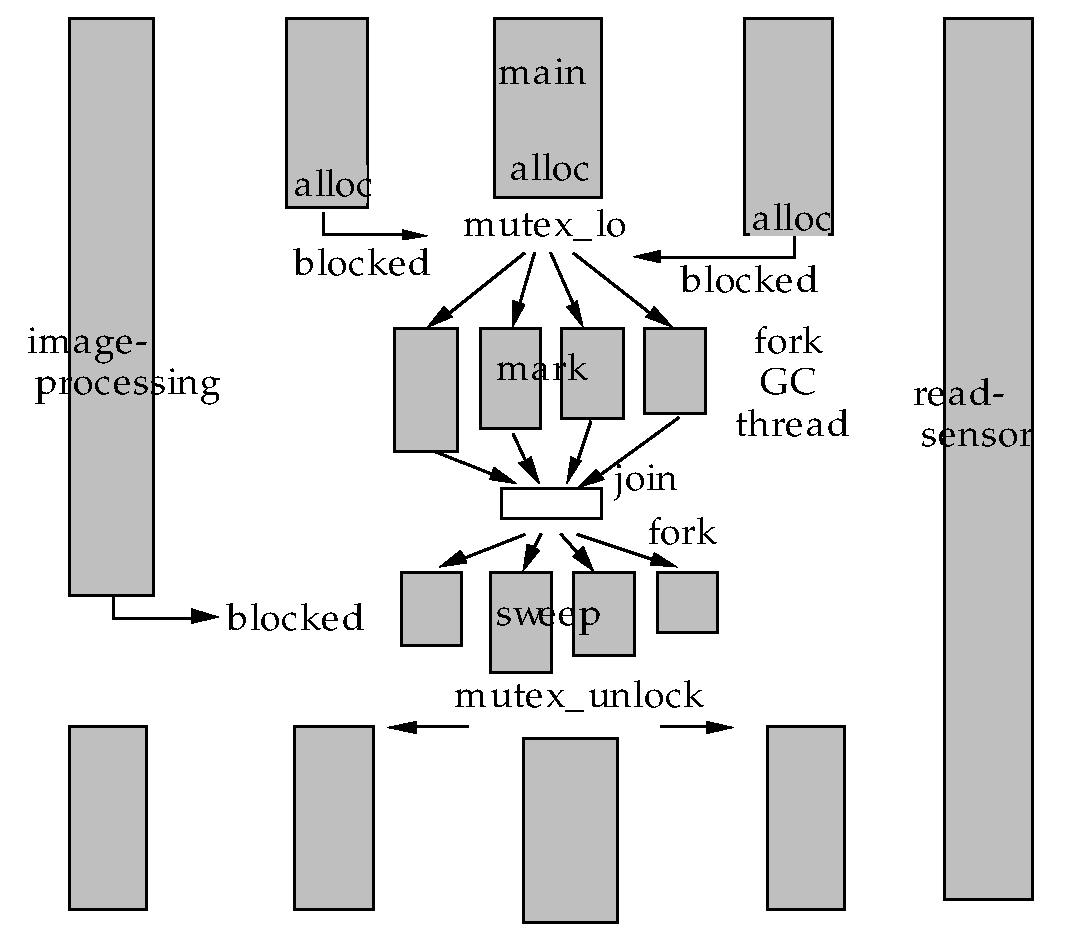
\includegraphics[width=120mm]{fig/parathreads.ps}%
\lthtmlpictureZ
\lthtmlcheckvsize\clearpage}

\stepcounter{subsection}
\stepcounter{subsubsection}
{\newpage\clearpage
\lthtmlpictureA{tex2html_wrap57684}%
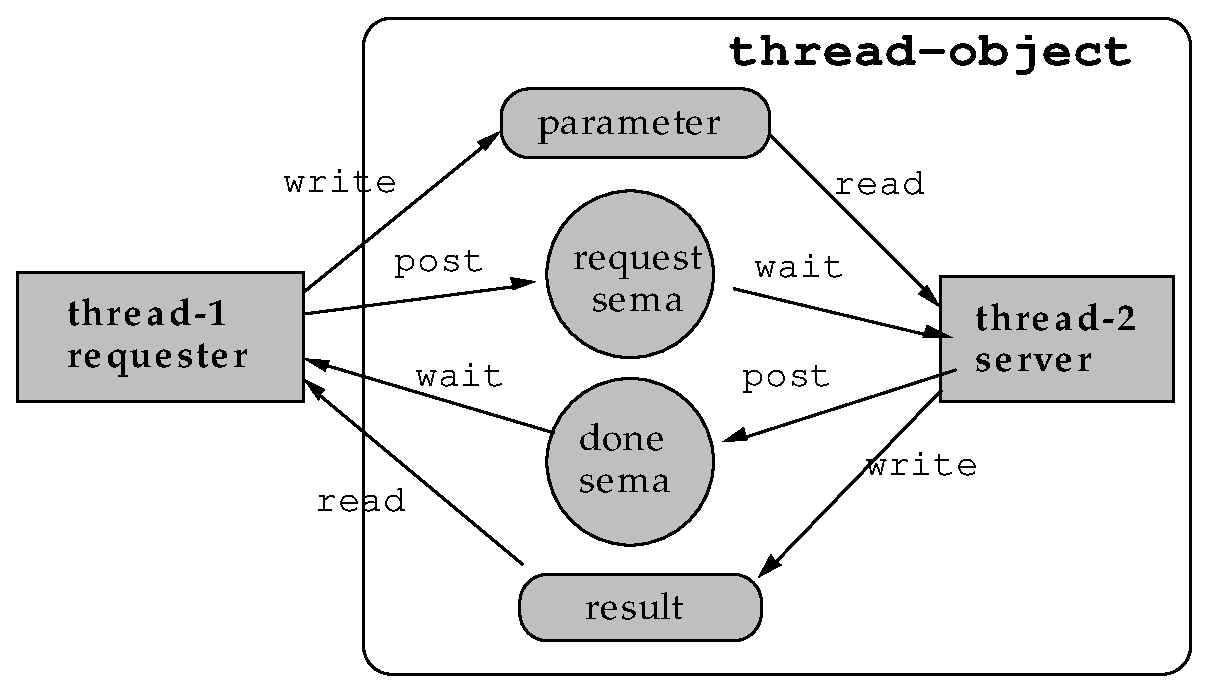
\includegraphics[width=7.5cm]{fig/threadobj.ps}%
\lthtmlpictureZ
\lthtmlcheckvsize\clearpage}

{\newpage\clearpage
\lthtmlpictureA{tex2html_wrap57686}%
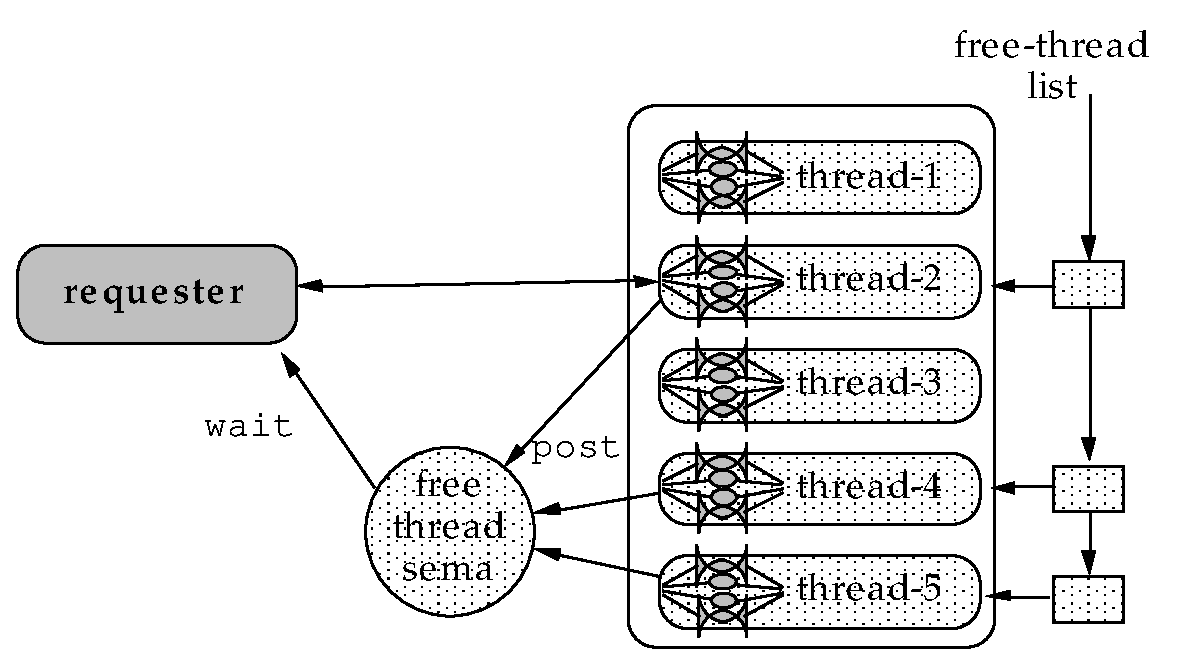
\includegraphics[width=7.5cm]{fig/threadpool.ps}%
\lthtmlpictureZ
\lthtmlcheckvsize\clearpage}

\stepcounter{subsubsection}
\stepcounter{subsubsection}
{\newpage\clearpage
\lthtmlpictureA{tex2html_wrap57695}%
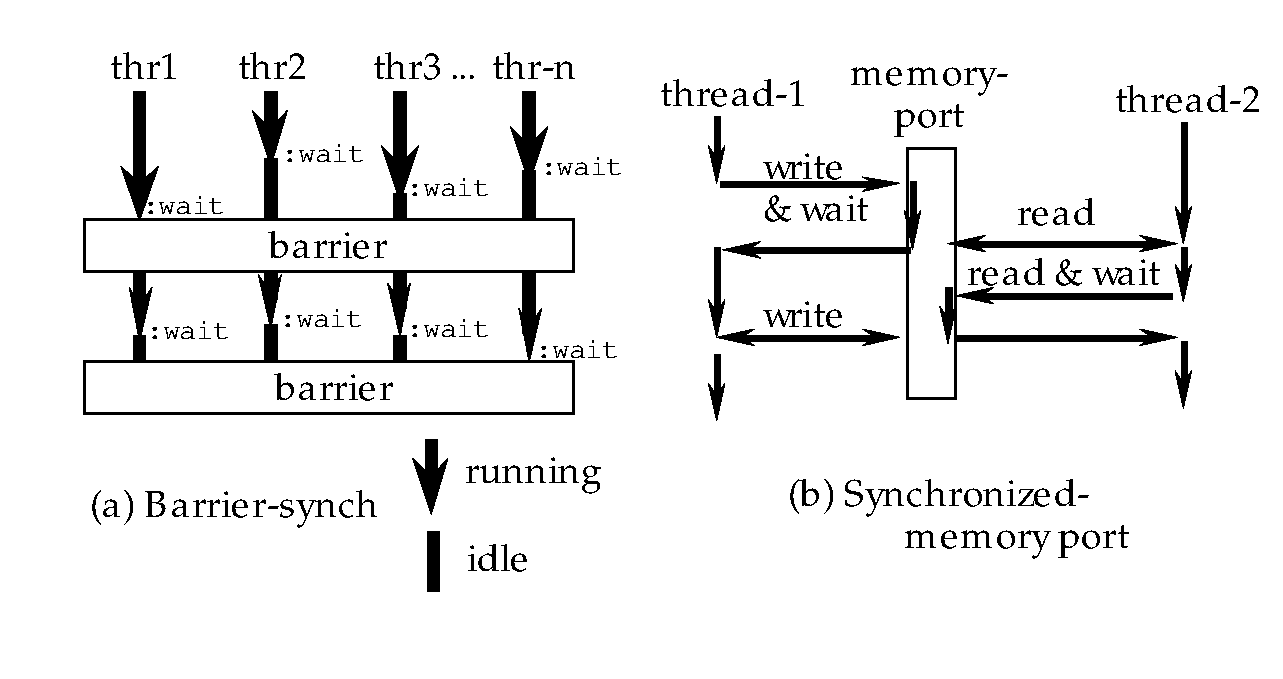
\includegraphics[width=130mm]{fig/synchports.ps}%
\lthtmlpictureZ
\lthtmlcheckvsize\clearpage}

\stepcounter{subsubsection}
\stepcounter{subsubsection}
\stepcounter{subsubsection}
\stepcounter{subsection}
\stepcounter{subsection}
\stepcounter{subsection}
\stepcounter{section}
\stepcounter{subsection}
\stepcounter{subsection}
\stepcounter{subsection}
\stepcounter{subsection}
\stepcounter{subsection}
\stepcounter{subsection}
{\newpage\clearpage
\lthtmlinlinemathA{tex2html_wrap_inline57923}%
$ 4\times4$%
\lthtmlinlinemathZ
\lthtmlcheckvsize\clearpage}

{\newpage\clearpage
\lthtmlinlinemathA{tex2html_wrap_indisplay57925}%
$\displaystyle T = \begin{pmatrix}
\mathbf{R}_T & \mathbf{p}_T \\
\mathbf{0} & 1
\end{pmatrix}
$%
\lthtmlindisplaymathZ
\lthtmlcheckvsize\clearpage}

{\newpage\clearpage
\lthtmlinlinemathA{tex2html_wrap_inline57927}%
$ \mathbf{R}_T$%
\lthtmlinlinemathZ
\lthtmlcheckvsize\clearpage}

{\newpage\clearpage
\lthtmlinlinemathA{tex2html_wrap_inline57929}%
$ 3\times3$%
\lthtmlinlinemathZ
\lthtmlcheckvsize\clearpage}

{\newpage\clearpage
\lthtmlinlinemathA{tex2html_wrap_inline57931}%
$ \mathbf{p}_T$%
\lthtmlinlinemathZ
\lthtmlcheckvsize\clearpage}

{\newpage\clearpage
\lthtmlinlinemathA{tex2html_wrap_inline57933}%
$ 3\times1$%
\lthtmlinlinemathZ
\lthtmlcheckvsize\clearpage}

{\newpage\clearpage
\lthtmlinlinemathA{tex2html_wrap_inline57935}%
$ \mathbf{R}$%
\lthtmlinlinemathZ
\lthtmlcheckvsize\clearpage}

{\newpage\clearpage
\lthtmlinlinemathA{tex2html_wrap_inline57946}%
$ \mathbf{p}$%
\lthtmlinlinemathZ
\lthtmlcheckvsize\clearpage}

{\newpage\clearpage
\lthtmlinlinemathA{tex2html_wrap_inline57948}%
$ \Rightarrow$%
\lthtmlinlinemathZ
\lthtmlcheckvsize\clearpage}

{\newpage\clearpage
\lthtmlinlinemathA{tex2html_wrap_inline57959}%
$ \mathbf{v}$%
\lthtmlinlinemathZ
\lthtmlcheckvsize\clearpage}

{\newpage\clearpage
\lthtmlinlinemathA{tex2html_wrap_inline57965}%
$ \mathbf{R}_T \mathbf{v}$%
\lthtmlinlinemathZ
\lthtmlcheckvsize\clearpage}

{\newpage\clearpage
\lthtmlinlinemathA{tex2html_wrap_inline57972}%
$ \mathbf{v}^T \mathbf{R}_T$%
\lthtmlinlinemathZ
\lthtmlcheckvsize\clearpage}

{\newpage\clearpage
\lthtmlinlinemathA{tex2html_wrap_inline57979}%
$ \mathbf{R}_T\mathbf{v} + \mathbf{p}_T$%
\lthtmlinlinemathZ
\lthtmlcheckvsize\clearpage}

{\newpage\clearpage
\lthtmlinlinemathA{tex2html_wrap_inline57986}%
$ \mathbf{R}_T^{-1}\left( \mathbf{v} - \mathbf{p}_T \right)$%
\lthtmlinlinemathZ
\lthtmlcheckvsize\clearpage}

{\newpage\clearpage
\lthtmlinlinemathA{tex2html_wrap_inline57992}%
$ T^{-1}$%
\lthtmlinlinemathZ
\lthtmlcheckvsize\clearpage}

{\newpage\clearpage
\lthtmlinlinemathA{tex2html_wrap_indisplay57994}%
$\displaystyle T^{-1} = \begin{pmatrix}
 \mathbf{R}_T^{-1} & -\mathbf{R}_T^{-1}\mathbf{p}_T \\
 \mathbf{0} & 1
\end{pmatrix}
$%
\lthtmlindisplaymathZ
\lthtmlcheckvsize\clearpage}

{\newpage\clearpage
\lthtmlinlinemathA{tex2html_wrap_inline57997}%
$ T^{-1}A$%
\lthtmlinlinemathZ
\lthtmlcheckvsize\clearpage}

{\newpage\clearpage
\lthtmlinlinemathA{tex2html_wrap_inline57999}%
$ AT^{-1}$%
\lthtmlinlinemathZ
\lthtmlcheckvsize\clearpage}

{\newpage\clearpage
\lthtmlinlinemathA{tex2html_wrap_inline58001}%
$ W^{-1}AT^{-1}W$%
\lthtmlinlinemathZ
\lthtmlcheckvsize\clearpage}

{\newpage\clearpage
\lthtmlinlinemathA{tex2html_wrap_inline58005}%
$ \Leftrightarrow$%
\lthtmlinlinemathZ
\lthtmlcheckvsize\clearpage}

{\newpage\clearpage
\lthtmlinlinemathA{tex2html_wrap_inline58007}%
$ \leftarrow$%
\lthtmlinlinemathZ
\lthtmlcheckvsize\clearpage}

{\newpage\clearpage
\lthtmlinlinemathA{tex2html_wrap_inline58009}%
$ \mathbf{R}_T \Leftrightarrow \mathbf{R}_A$%
\lthtmlinlinemathZ
\lthtmlcheckvsize\clearpage}

{\newpage\clearpage
\lthtmlinlinemathA{tex2html_wrap_inline58011}%
$ \mathbf{p}_T \Leftrightarrow \mathbf{p}_A$%
\lthtmlinlinemathZ
\lthtmlcheckvsize\clearpage}

{\newpage\clearpage
\lthtmlinlinemathA{tex2html_wrap_inline58018}%
$ \mathbf{R}_T \Leftrightarrow \mathbf{R}$%
\lthtmlinlinemathZ
\lthtmlcheckvsize\clearpage}

{\newpage\clearpage
\lthtmlinlinemathA{tex2html_wrap_inline58020}%
$ \mathbf{p}_T \Leftrightarrow \mathbf{p}$%
\lthtmlinlinemathZ
\lthtmlcheckvsize\clearpage}

{\newpage\clearpage
\lthtmlinlinemathA{tex2html_wrap_inline58023}%
$ T \leftarrow TA$%
\lthtmlinlinemathZ
\lthtmlcheckvsize\clearpage}

{\newpage\clearpage
\lthtmlinlinemathA{tex2html_wrap_inline58025}%
$ T \Leftrightarrow A$%
\lthtmlinlinemathZ
\lthtmlcheckvsize\clearpage}

{\newpage\clearpage
\lthtmlinlinemathA{tex2html_wrap_inline58027}%
$ T \leftarrow WA$%
\lthtmlinlinemathZ
\lthtmlcheckvsize\clearpage}

{\newpage\clearpage
\lthtmlinlinemathA{tex2html_wrap_inline58032}%
$ \mathbf{p}_{T} \leftarrow \mathbf{p}_{T} + \mathbf{R}_{T}\mathbf{v}$%
\lthtmlinlinemathZ
\lthtmlcheckvsize\clearpage}

{\newpage\clearpage
\lthtmlinlinemathA{tex2html_wrap_inline58034}%
$ \mathbf{p}_{T} \leftarrow \mathbf{p}_{T} + \mathbf{v}$%
\lthtmlinlinemathZ
\lthtmlcheckvsize\clearpage}

{\newpage\clearpage
\lthtmlinlinemathA{tex2html_wrap_inline58036}%
$ \mathbf{p}_{T} \leftarrow \mathbf{p}_{T} + \mathbf{R}_{W}\mathbf{v}$%
\lthtmlinlinemathZ
\lthtmlcheckvsize\clearpage}

{\newpage\clearpage
\lthtmlinlinemathA{tex2html_wrap_inline58043}%
$ \mathbf{p}_{T} \leftarrow \mathbf{v}$%
\lthtmlinlinemathZ
\lthtmlcheckvsize\clearpage}

{\newpage\clearpage
\lthtmlinlinemathA{tex2html_wrap_inline58045}%
$ \mathbf{p}_{T} \leftarrow \mathbf{p}_{W} + \mathbf{R}_{W}\mathbf{v}$%
\lthtmlinlinemathZ
\lthtmlcheckvsize\clearpage}

{\newpage\clearpage
\lthtmlinlinemathA{tex2html_wrap_inline58050}%
$ T \leftarrow AT$%
\lthtmlinlinemathZ
\lthtmlcheckvsize\clearpage}

{\newpage\clearpage
\lthtmlinlinemathA{tex2html_wrap_inline58052}%
$ T \leftarrow$%
\lthtmlinlinemathZ
\lthtmlcheckvsize\clearpage}

{\newpage\clearpage
\lthtmlinlinemathA{tex2html_wrap_inline58054}%
$ \left( WAW \right)^{-1} T$%
\lthtmlinlinemathZ
\lthtmlcheckvsize\clearpage}

\stepcounter{section}
{\newpage\clearpage
\lthtmlpictureA{tex2html_wrap58057}%
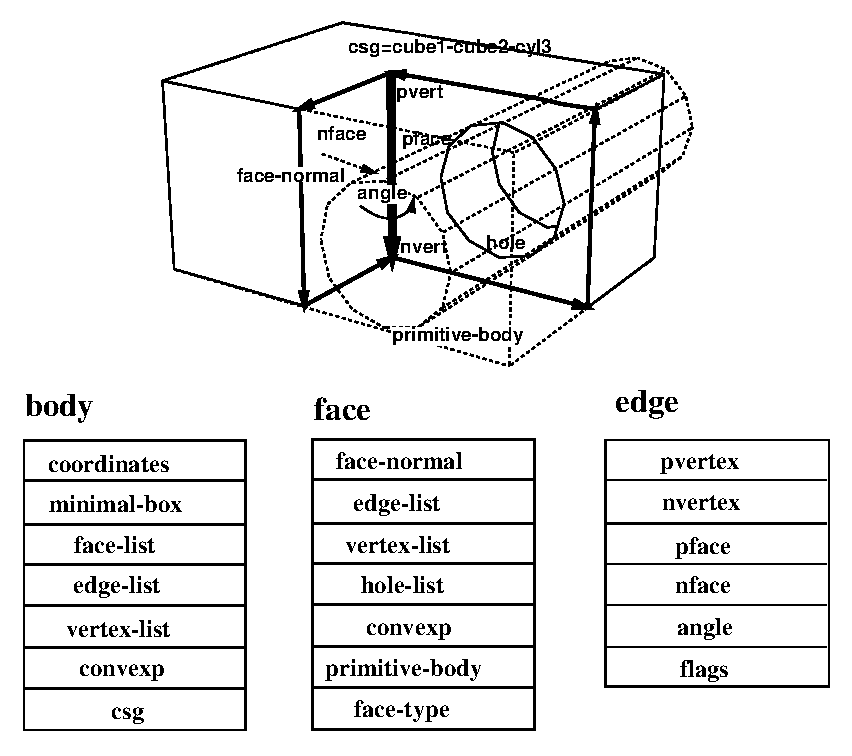
\includegraphics[height=10cm]{fig/beam.ps}%
\lthtmlpictureZ
\lthtmlcheckvsize\clearpage}

\stepcounter{subsection}
\stepcounter{subsection}
\stepcounter{subsection}
\stepcounter{subsection}
\stepcounter{subsection}
{\newpage\clearpage
\lthtmlpictureA{tex2html_wrap58278}%
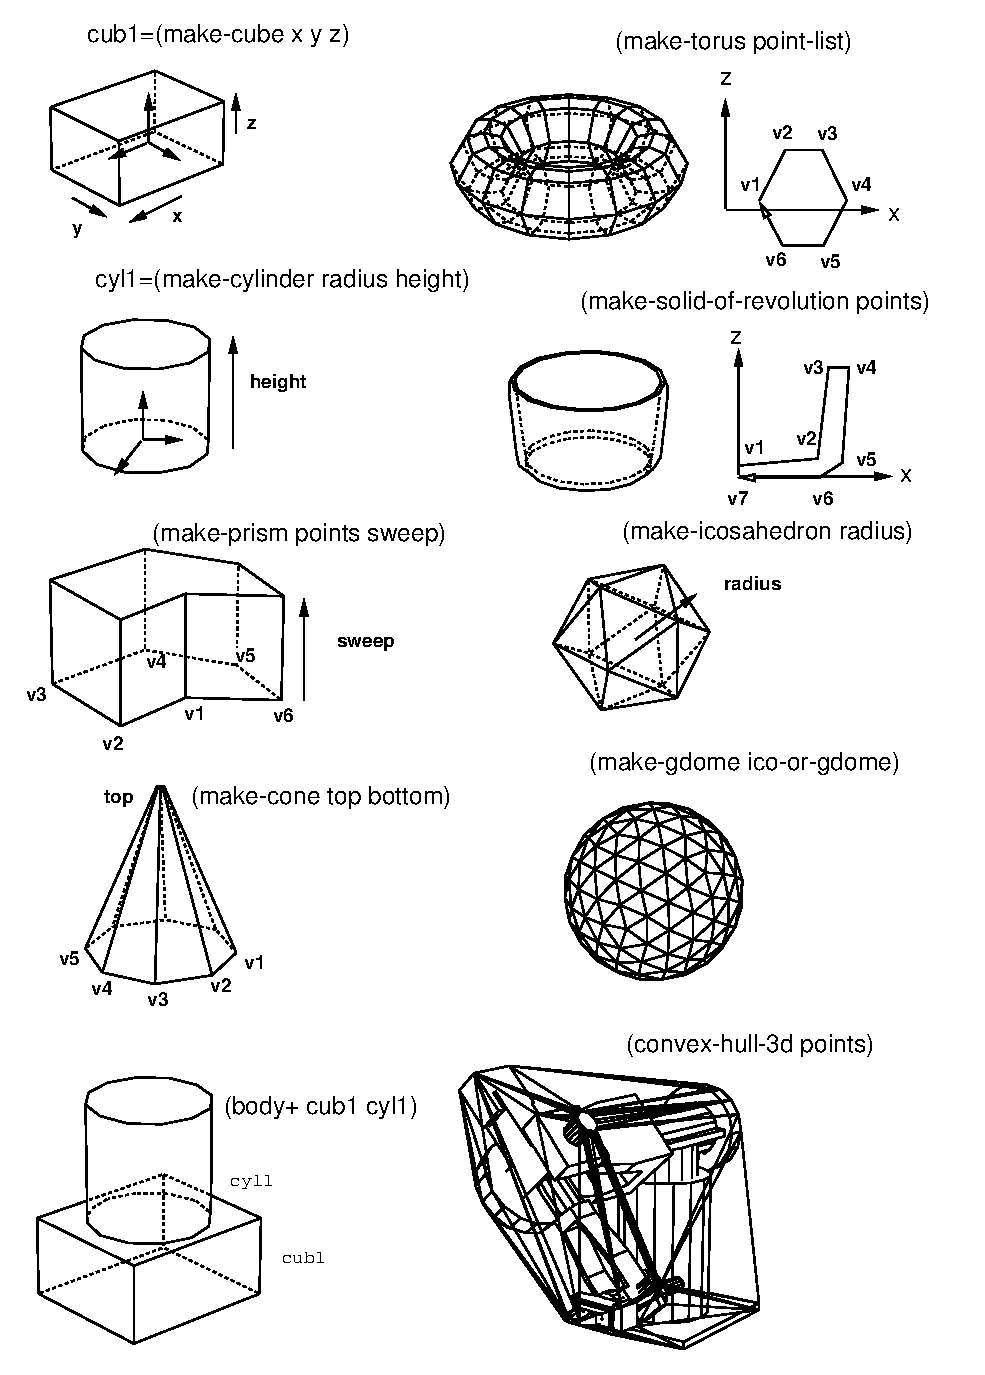
\includegraphics[height=19cm]{fig/fig1.ps}%
\lthtmlpictureZ
\lthtmlcheckvsize\clearpage}

\stepcounter{subsection}
\stepcounter{subsection}
\stepcounter{subsection}
{\newpage\clearpage
\lthtmlpictureA{tex2html_wrap58318}%
\includegraphics[width=7.9cm]{fig/fig-peg-in-hole1.ps}%
\lthtmlpictureZ
\lthtmlcheckvsize\clearpage}

{\newpage\clearpage
\lthtmlpictureA{tex2html_wrap58319}%
\includegraphics[width=7.9cm]{fig/fig-peg-in-hole2.ps}%
\lthtmlpictureZ
\lthtmlcheckvsize\clearpage}

{\newpage\clearpage
\lthtmlpictureA{tex2html_wrap58320}%
\includegraphics[width=7.9cm]{fig/fig-peg-in-hole3.ps}%
\lthtmlpictureZ
\lthtmlcheckvsize\clearpage}

{\newpage\clearpage
\lthtmlpictureA{tex2html_wrap58321}%
\includegraphics[width=7.9cm]{fig/fig-peg-in-hole4.ps}%
\lthtmlpictureZ
\lthtmlcheckvsize\clearpage}

{\newpage\clearpage
\lthtmlpictureA{tex2html_wrap58322}%
\includegraphics[width=7.9cm]{fig/fig-peg-naname-m1.ps}%
\lthtmlpictureZ
\lthtmlcheckvsize\clearpage}

{\newpage\clearpage
\lthtmlpictureA{tex2html_wrap58323}%
\includegraphics[width=7.9cm]{fig/fig-peg-naname-m2.ps}%
\lthtmlpictureZ
\lthtmlcheckvsize\clearpage}

{\newpage\clearpage
\lthtmlpictureA{tex2html_wrap58324}%
\includegraphics[width=7.9cm]{fig/fig-peg-naname-m3.ps}%
\lthtmlpictureZ
\lthtmlcheckvsize\clearpage}

{\newpage\clearpage
\lthtmlpictureA{tex2html_wrap58325}%
\includegraphics[width=7.9cm]{fig/fig-peg-naname-m4.ps}%
\lthtmlpictureZ
\lthtmlcheckvsize\clearpage}

\stepcounter{subsection}
\stepcounter{section}
\stepcounter{subsection}
{\newpage\clearpage
\lthtmlpictureA{tex2html_wrap58349}%
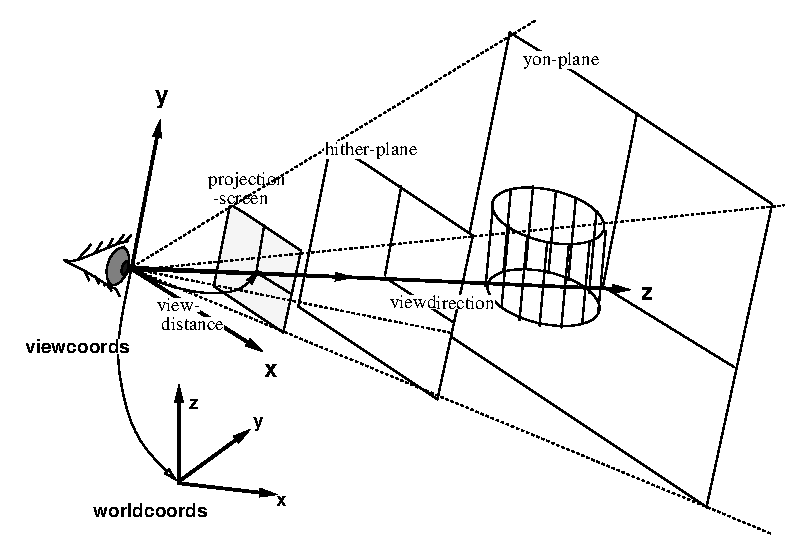
\includegraphics[height=10cm]{fig/viewcoords.ps}%
\lthtmlpictureZ
\lthtmlcheckvsize\clearpage}

\stepcounter{subsection}
\stepcounter{subsection}
\stepcounter{subsection}
\stepcounter{subsection}
\stepcounter{subsection}
\stepcounter{section}
\stepcounter{subsection}
\stepcounter{subsection}
{\newpage\clearpage
\lthtmlpictureA{tex2html_wrap58507}%
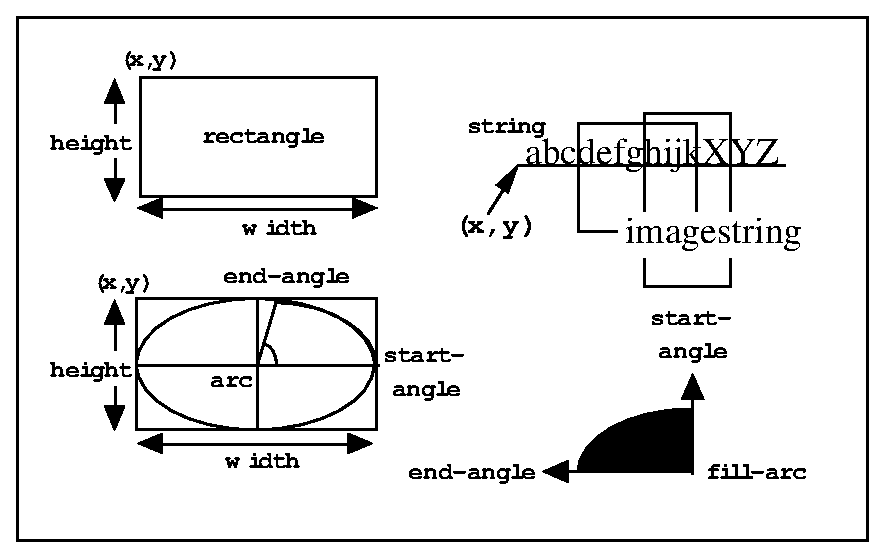
\includegraphics[height=6cm]{fig/xdraw.ps}%
\lthtmlpictureZ
\lthtmlcheckvsize\clearpage}

\stepcounter{subsection}
\stepcounter{subsection}
\stepcounter{section}
\stepcounter{subsection}
\stepcounter{subsection}
{\newpage\clearpage
\lthtmlpictureA{tex2html_wrap58645}%
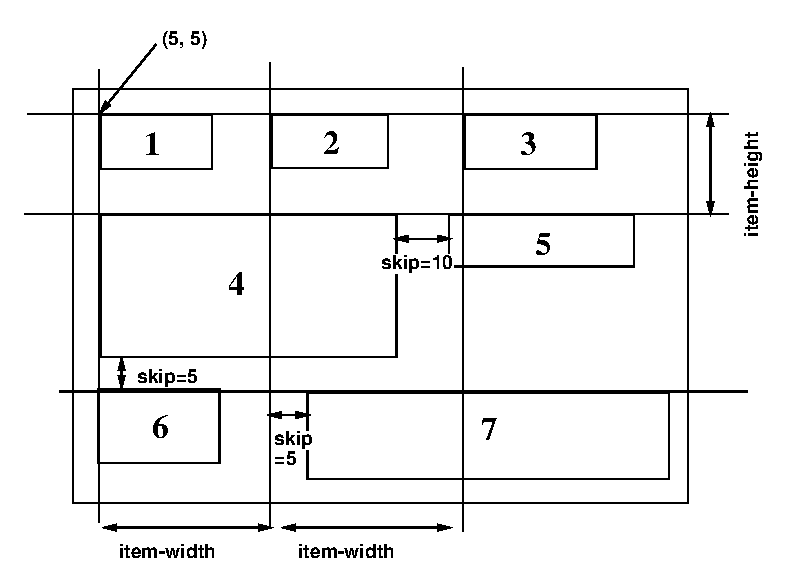
\includegraphics[height=7cm]{fig/panellayout.ps}%
\lthtmlpictureZ
\lthtmlcheckvsize\clearpage}

\stepcounter{subsubsection}
\stepcounter{subsubsection}
{\newpage\clearpage
\lthtmlpictureA{tex2html_wrap58666}%
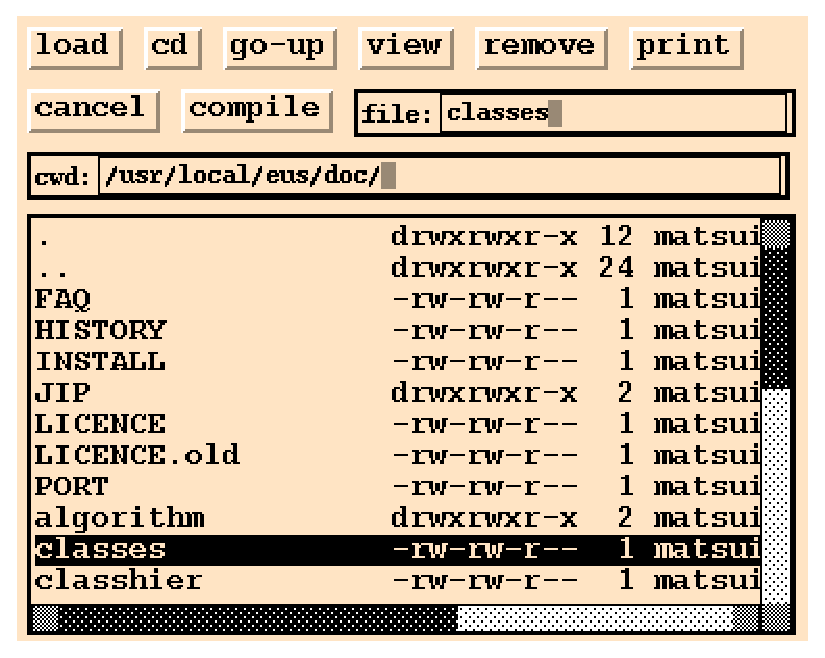
\includegraphics[height=7.5cm]{fig/filepanel.ps}%
\lthtmlpictureZ
\lthtmlcheckvsize\clearpage}

\stepcounter{subsubsection}
{\newpage\clearpage
\lthtmlpictureA{tex2html_wrap58671}%
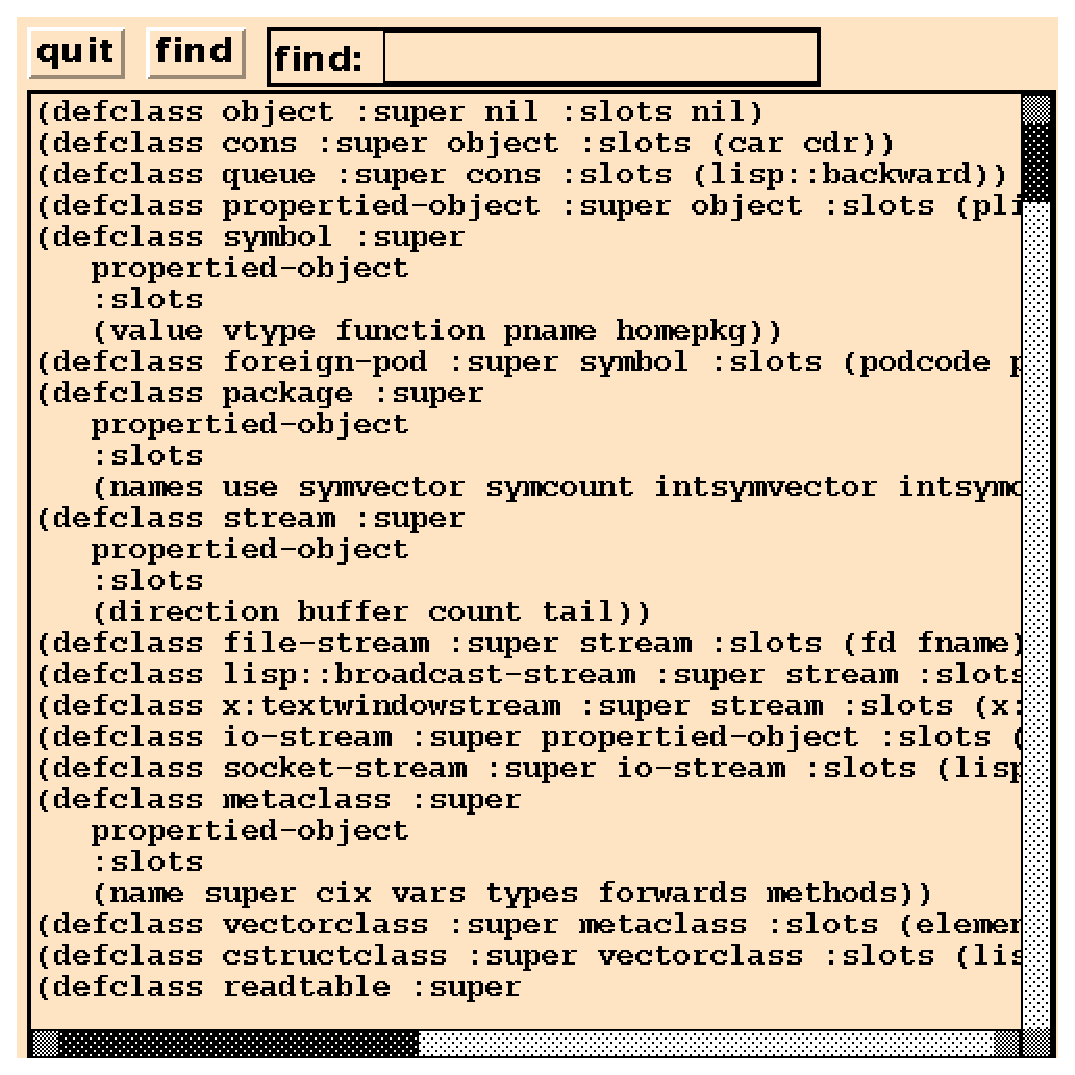
\includegraphics[height=7cm]{fig/textviewpanel.ps}%
\lthtmlpictureZ
\lthtmlcheckvsize\clearpage}

\stepcounter{subsection}
{\newpage\clearpage
\lthtmlpictureA{tex2html_wrap58704}%
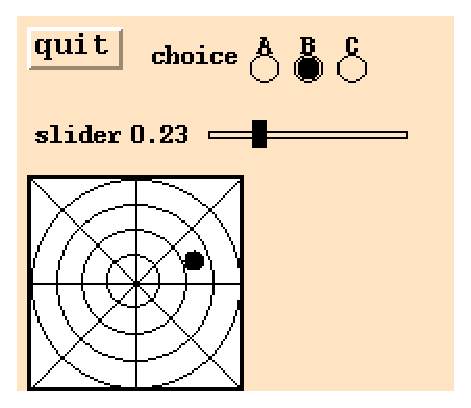
\includegraphics[height=5cm]{fig/panelitem.ps}%
\lthtmlpictureZ
\lthtmlcheckvsize\clearpage}

\stepcounter{subsection}
\stepcounter{subsection}
\stepcounter{section}
\stepcounter{subsection}
\stepcounter{subsection}
\stepcounter{subsection}
\stepcounter{subsection}
{\newpage\clearpage
\lthtmlpictureA{tex2html_wrap58858}%
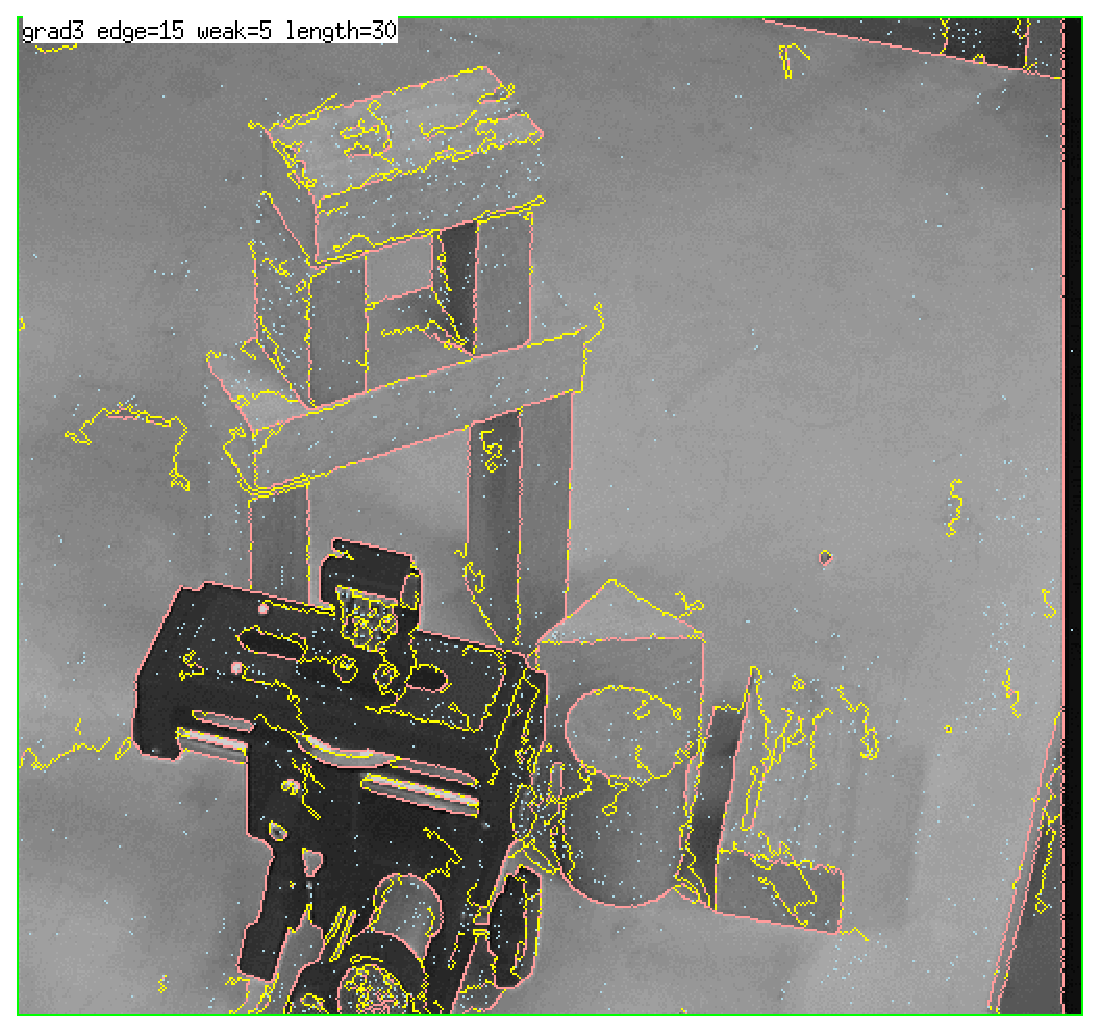
\includegraphics[height=9cm]{fig/block1.edg.ps}%
\lthtmlpictureZ
\lthtmlcheckvsize\clearpage}

\stepcounter{subsection}
\stepcounter{subsection}
\stepcounter{section}
\stepcounter{subsection}
\stepcounter{subsection}
{\newpage\clearpage
\lthtmldisplayA{displaymath58918}%
\begin{displaymath}
\begin{array}{ll}
T & = base \cdot J1 \cdot J2 \cdot \ldots 
\cdot J6 \cdot handcoords \cdot toolcoords \\
 & = (send \; eta3 \; :worldcoords) \\
T_{Jn} & = base \cdot J1\cdot \ldots \cdot Jn \\
 & = (send \; Jn \; :worldcoords) \\
T_{arm} & = J1 \cdot J2 \cdot \ldots \cdot J6 \cdot handcoords \\
 & = (send \; eta3 \; :armsol-coords) \\
T_{tool} & = J1 \cdot J2 \cdot  \ldots \cdot J6 \cdot handcoords \cdot toolcoords \\
 & = (send \; eta3 \; :copy-coords) \\
T_{t} & = toolcoords \\
 & = (manipulator-toolcoords \; eta3)\\
T_{t}^{-1} & = toolcoords^{-1} \\
 & = (manipulator-toolinverse \; eta3) \\
T_{h} & = handcoords \\
 & = (manipulator-handcoords \; eta3)\\
\end{array}\end{displaymath}%
\lthtmldisplayZ
\lthtmlcheckvsize\clearpage}

{\newpage\clearpage
\lthtmlpictureA{tex2html_wrap58921}%
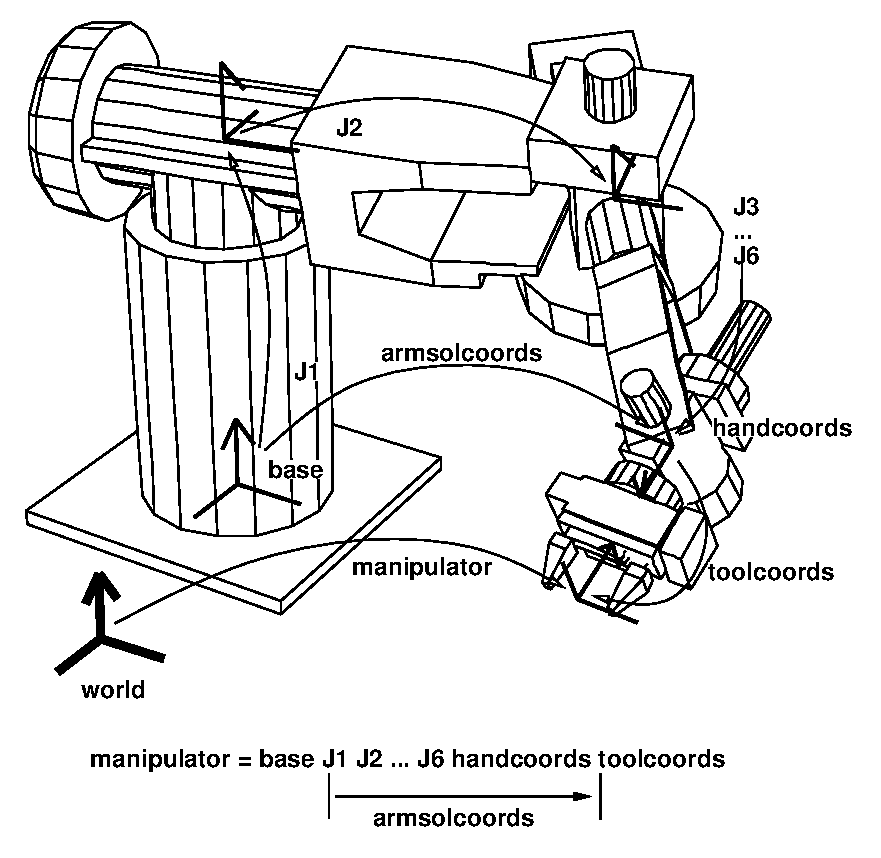
\includegraphics[height=100mm]{fig/eta3coords.ps}%
\lthtmlpictureZ
\lthtmlcheckvsize\clearpage}

\stepcounter{section}
\stepcounter{subsection}
\stepcounter{subsection}
{\newpage\clearpage
\lthtmlpictureA{tex2html_wrap58939}%
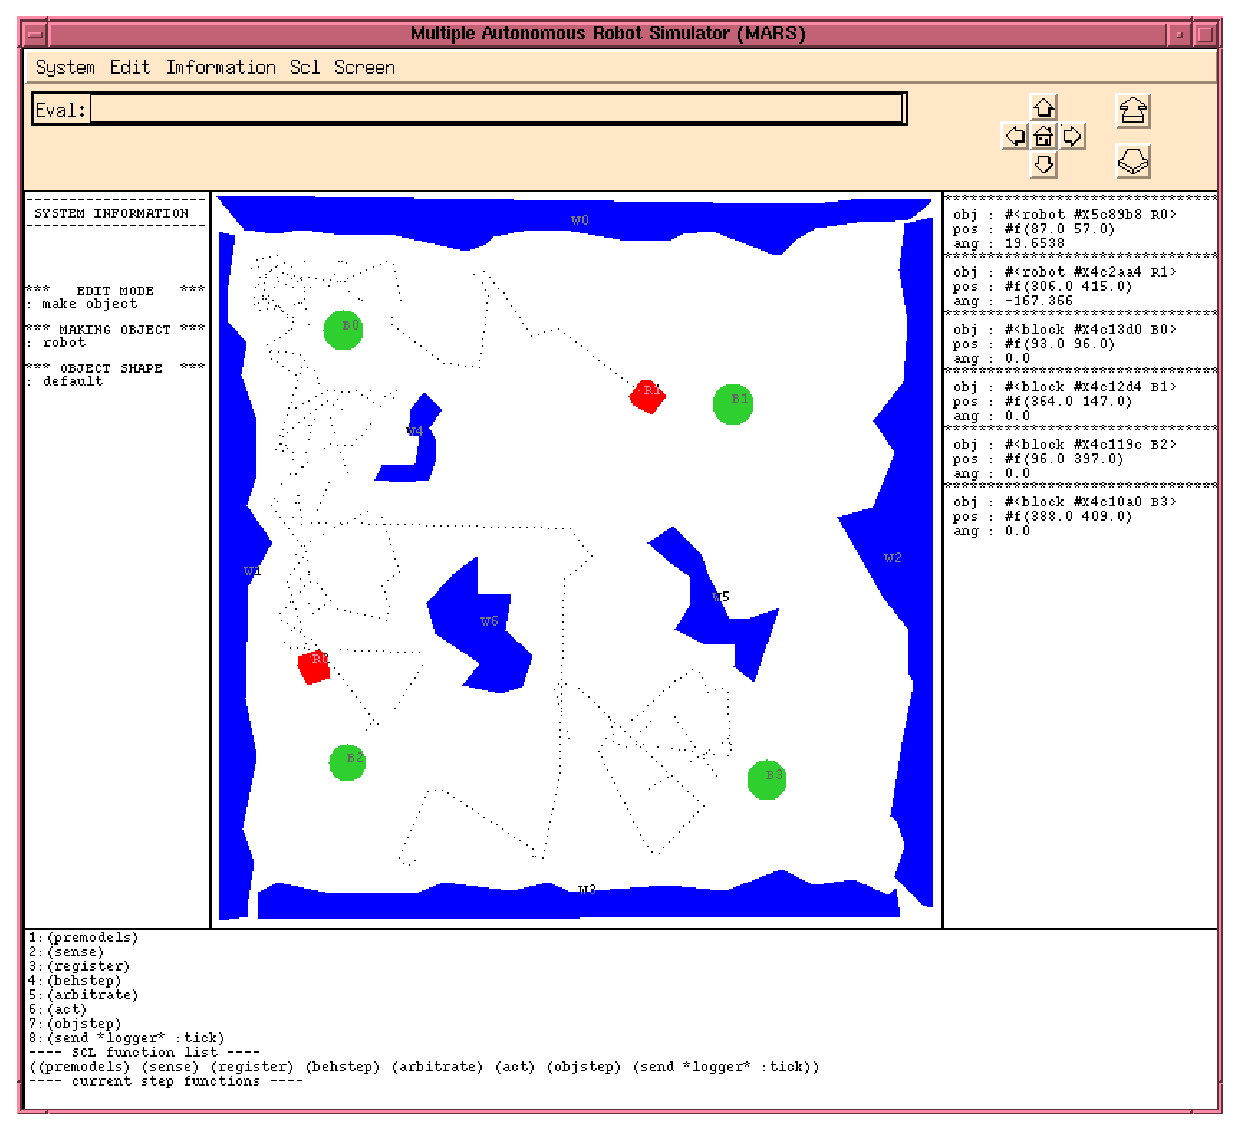
\includegraphics[width=0.4\columnwidth]{fig/mars.eps}%
\lthtmlpictureZ
\lthtmlcheckvsize\clearpage}

{\newpage\clearpage
\lthtmlpictureA{tex2html_wrap58941}%
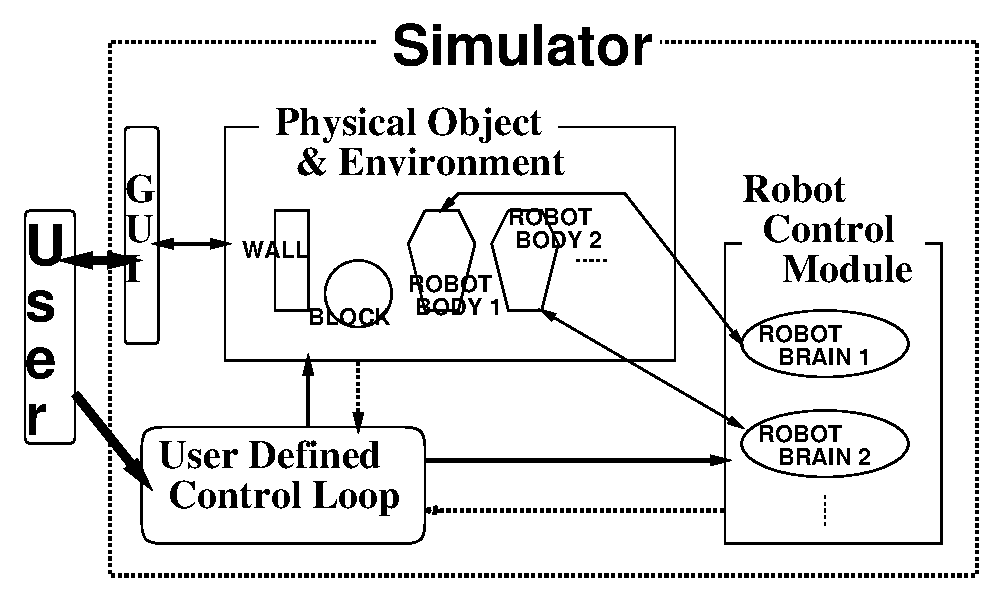
\includegraphics[width=0.6\columnwidth]{fig/simst.ps}%
\lthtmlpictureZ
\lthtmlcheckvsize\clearpage}

{\newpage\clearpage
\lthtmlpictureA{tex2html_wrap58946}%
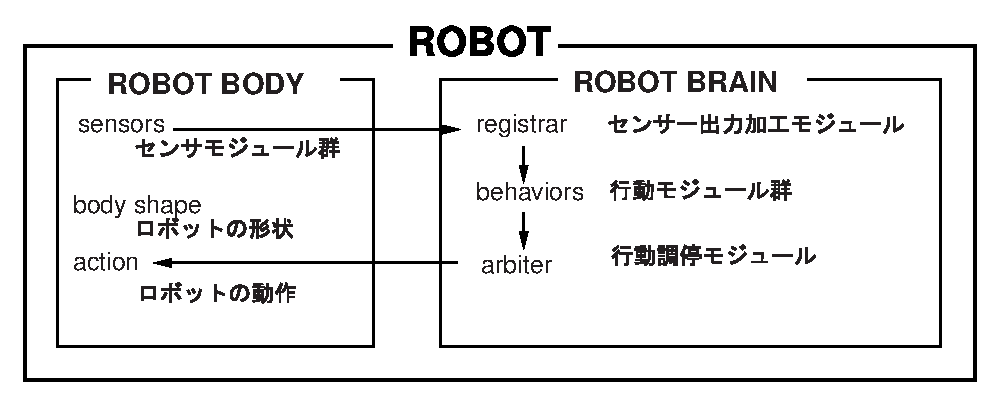
\includegraphics[width=0.5\columnwidth]{fig/robot-ui2.ps}%
\lthtmlpictureZ
\lthtmlcheckvsize\clearpage}

{\newpage\clearpage
\lthtmlpictureA{tex2html_wrap58948}%
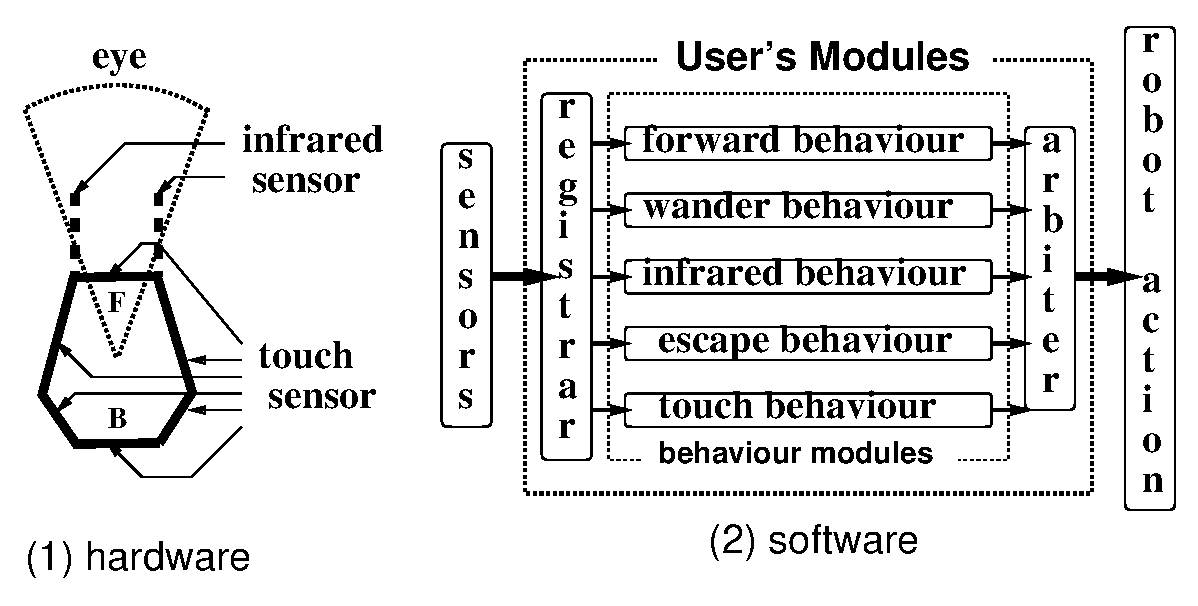
\includegraphics[width=0.5\columnwidth]{fig/robot-st2.ps}%
\lthtmlpictureZ
\lthtmlcheckvsize\clearpage}


\end{document}
